\section{Pruebas en simulación}

Las pruebas en simulación se ejecutan en el entorno virtual desarrollado en Unreal Engine 5, con sensores y dinámica equivalentes al sistema propuesto. Esta instancia permite validar desempeño de navegación y percepción en condiciones controladas antes de la campaña experimental sobre hardware.

\subsection{Estructura de documentación de pruebas}

Todas las pruebas de este capítulo siguen la misma estructura:
\begin{itemize}
    \item \textbf{Descripción de la prueba:} objetivo técnico y alcance.
    \item \textbf{Criterios de aprobación:} umbrales mínimos de desempeño.
    \item \textbf{Procedimiento de ejecución:} secuencia de pasos y parámetros de corrida.
    \item \textbf{Resultados:} métricas medidas y veredicto de cumplimiento.
\end{itemize}

\subsection{Calidad de mapeo con LiDAR simulado}

\subsubsection{Descripción de la prueba}

Esta prueba evalúa de forma aislada la capacidad del módulo SLAM para construir un mapa de ocupación preciso y completo a partir del LiDAR simulado, sin considerar la calidad de navegación ni eventos externos. El robot recorre un entorno virtual cerrado con geometría conocida, y el mapa generado se compara contra el mapa de referencia del escenario.

\paragraph{Objetivos mínimos}
\begin{itemize}
    \item Verificar que el mapa cubre la totalidad del área navegable del entorno.
    \item Validar la precisión geométrica del mapa respecto al mapa de referencia.
    \item Medir la velocidad de convergencia del mapa durante el barrido.
    \item Cuantificar errores de clasificación de celdas (falsas ocupaciones).
\end{itemize}

\subsubsection{Criterios de aprobación}

\begin{table}[H]
\centering
\small
\begin{tabular}{p{8.8cm} p{4.1cm}}
\toprule
\textbf{Métrica} & \textbf{Criterio de aprobación} \\
\midrule
Calidad del mapa de ocupación (IoU mapa generado vs mapa de referencia) & $\geq 0{,}75$ \\
Cobertura del área navegable en el mapa generado & $\geq 90\%$ \\
Porcentaje de celdas libres clasificadas erróneamente como ocupadas & $\leq 5\%$ \\
Tiempo de convergencia del mapa (IoU $\geq 0{,}70$ estable por $\geq 10\ \text{s}$) & $\leq 5\ \text{min}$ \\
Entropía media de la grilla al finalizar el barrido & $\leq 0{,}15\ \text{bits/celda}$ \\
\bottomrule
\end{tabular}
\caption{Criterios de aprobación de la prueba de mapeo con LiDAR simulado.}
\label{tab:criterios_prueba_slam}
\end{table}

\subsubsection{Procedimiento de ejecución}

\begin{enumerate}
    \item Configurar escenario virtual cerrado con geometría conocida y exportar mapa de referencia en formato de grilla de ocupación 2D, con resolución de celda de $0{,}15\ \text{m}$.
    \item Inicializar el robot en posición de inicio conocida con módulo SLAM activo y LiDAR simulado habilitado.
    \item Ejecutar un barrido manual o teleoperado del entorno completo, sin activar planificación de trayectoria autónoma.
    \item Registrar el estado del mapa a intervalos de 10 s: IoU parcial, cobertura y entropía de la grilla.
    \item Al finalizar el barrido, exportar el mapa generado y compararlo contra el mapa de referencia.
    \item Calcular la tasa de celdas libres mal clasificadas (falsos positivos de ocupación).
    \item Determinar el instante en que el IoU superó $0{,}70$ de forma estable y registrarlo como tiempo de convergencia.
\end{enumerate}

\subsubsection{Resultados}

\begin{table}[H]
\centering
\small
\begin{tabular}{p{8.8cm} p{2.2cm} p{2.8cm}}
\toprule
\textbf{Métrica} & \textbf{Resultado} & \textbf{Cumple} \\
\midrule
IoU mapa generado vs referencia [-] & 0,81 & Sí \\
Cobertura del mapa navegable [\%] & 95,3 & Sí \\
Celdas libres mal clasificadas [\%] & 4,7 & Sí \\
Tiempo de convergencia del mapa [min:s] & 3:12 & Sí \\
Entropía media de la grilla [bits/celda] & 0,08 & Sí \\
\bottomrule
\end{tabular}
\caption{Resultados medidos de la prueba de mapeo con LiDAR simulado.}
\label{tab:resultados_prueba_slam}
\end{table}

El barrido del entorno MissionA produjo un mapa de ocupación 2D con resolución de celda de $0{,}15\ \text{m}$, IoU de 0,81 respecto del mapa de referencia y cobertura del 95,3\% del área navegable. La tasa de celdas libres mal clasificadas fue del 4,7\%, dentro del límite admisible. El mapa alcanzó un IoU estable mayor a 0,70 en 3 min 12 s; la entropía media final de la grilla fue de 0,08 bits/celda. La Figura~\ref{fig:prueba_slam_mapas} contrasta ambos mapas en coordenadas métricas; la Figura~\ref{fig:prueba_slam_iou} registra la evolución del IoU durante el barrido.

\begin{figure}[H]
\centering
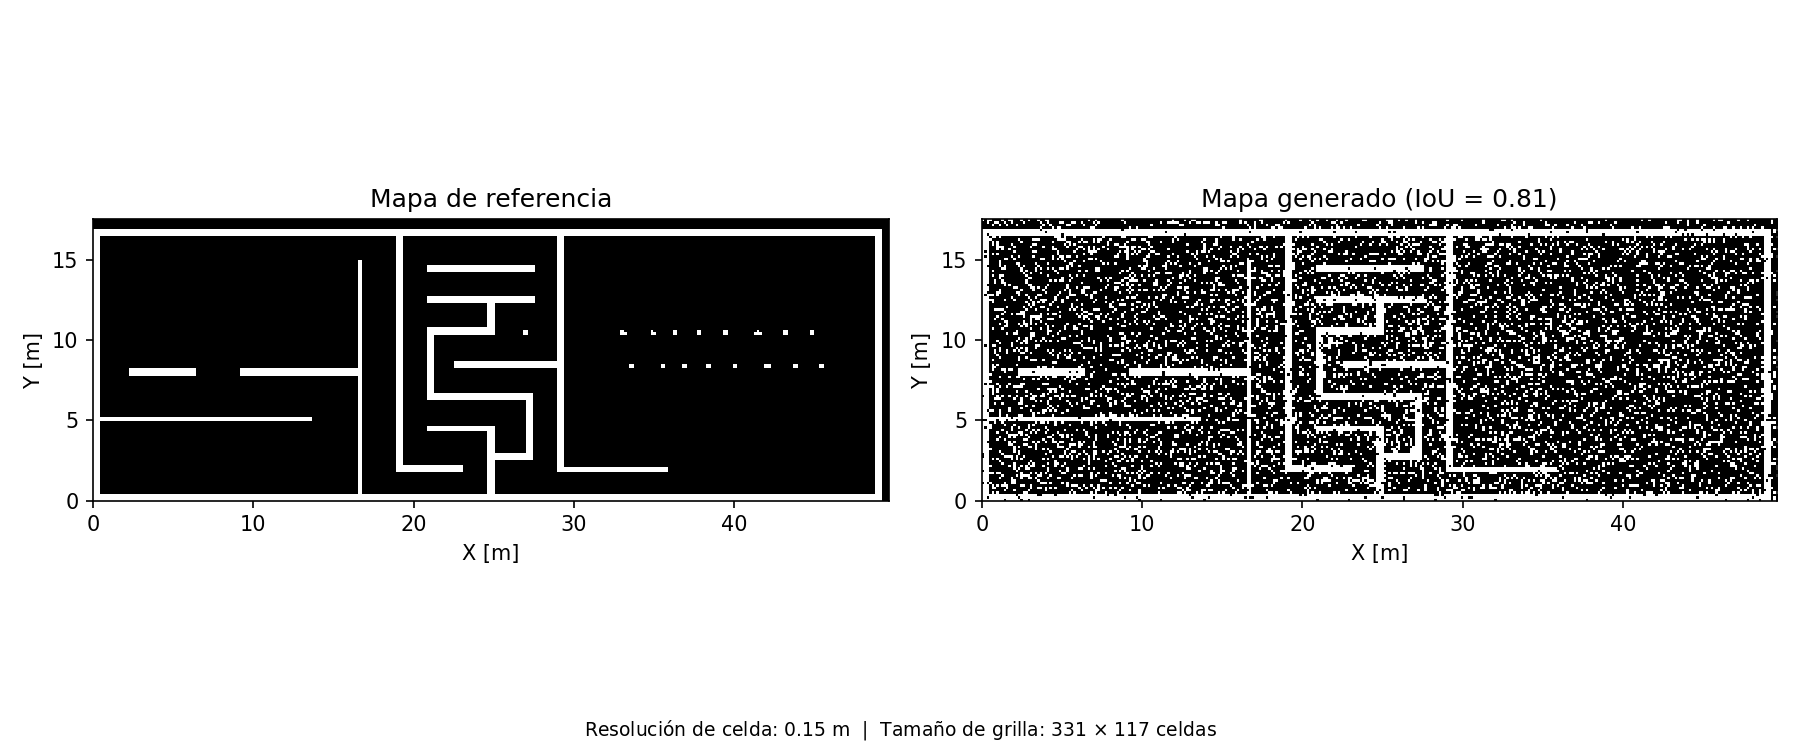
\includegraphics[width=.95\textwidth]{Figures/prueba_slam_mapas.png}
\caption{Comparación entre mapa de referencia del escenario y mapa de ocupación 2D generado por el módulo SLAM (celda de $0{,}15\ \text{m}$).}
\label{fig:prueba_slam_mapas}
\end{figure}

\begin{figure}[H]
\centering
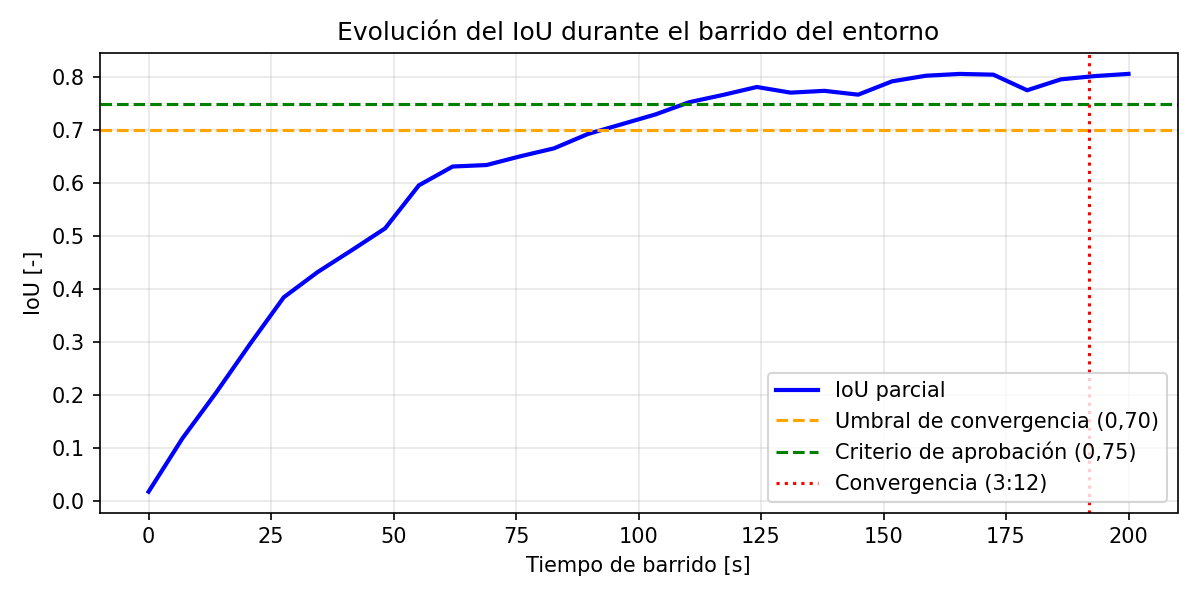
\includegraphics[width=.9\textwidth]{Figures/prueba_slam_convergencia_iou.png}
\caption{Evolución del índice IoU durante el barrido del entorno.}
\label{fig:prueba_slam_iou}
\end{figure}

\subsection{Planificación y seguimiento de trayectoria en simulación}

\subsubsection{Descripción de la prueba}

Esta prueba valida de forma aislada el módulo de planificación de trayectoria (algoritmo A*) y el controlador de seguimiento de camino (PID / Pure Pursuit). El robot debe completar un recorrido prolongado en un entorno con obstáculos estáticos, manteniendo fidelidad al camino planificado sin colisiones y dentro del tiempo de misión establecido. No se inyectan eventos dinámicos ni ruido de localización global.

Tomando una longitud de robot de $L_r = 0{,}60\ \text{m}$, la distancia mínima de prueba queda definida como:
\[
D_{\min} = 200 \cdot L_r = 120\ \text{m}
\]

\paragraph{Objetivos mínimos}
\begin{itemize}
    \item Completar una trayectoria de al menos $120\ \text{m}$ sin colisiones con obstáculos estáticos.
    \item Verificar que el controlador de seguimiento mantiene el robot dentro de la banda lateral admisible.
    \item Evaluar la suavidad de la trayectoria ejecutada y la cantidad de replanificaciones generadas.
\end{itemize}

\subsubsection{Criterios de aprobación}

\begin{table}[H]
\centering
\small
\begin{tabular}{p{8.8cm} p{4.1cm}}
\toprule
\textbf{Métrica} & \textbf{Criterio de aprobación} \\
\midrule
Distancia total recorrida & $\geq 120\ \text{m}$ \\
Tiempo total para completar el recorrido & $\leq 10\ \text{min}$ \\
Colisiones con obstáculos estáticos & 0 eventos \\
Desviación lateral media respecto al camino planificado & $\leq 0{,}15\ \text{m}$ \\
Desviación lateral máxima en tramo de corredor estrecho & $\leq 0{,}30\ \text{m}$ \\
Cantidad de replanificaciones de ruta durante la misión & $\leq 3$ \\
Varianza de curvatura de la trayectoria ejecutada & $\leq 0{,}10\ \text{m}^{-2}$ \\
\bottomrule
\end{tabular}
\caption{Criterios de aprobación de la prueba de planificación y seguimiento de trayectoria.}
\label{tab:criterios_prueba_path_planning}
\end{table}

\subsubsection{Procedimiento de ejecución}

\begin{enumerate}
    \item Configurar escenario virtual con obstáculos estáticos, al menos un corredor estrecho y un tramo abierto para navegación prolongada.
    \item Definir ruta de misión de al menos $120\ \text{m}$ con waypoints distribuidos en el entorno.
    \item Inicializar el robot en estado \texttt{NAVIGATING} con planificación autónoma activa, localización exacta (sin ruido) y mapeo desactivado para aislar el módulo de control.
    \item Activar registro de trayectoria de referencia, trayectoria ejecutada, tiempos de estado y eventos de colisión.
    \item Al detectar obstáculo imprevisto, registrar si el planificador genera una nueva ruta y contabilizarla.
    \item Calcular desviación lateral punto a punto entre trayectoria ejecutada y trayectoria planificada.
    \item Calcular la curvatura de la trayectoria ejecutada y su varianza como indicador de suavidad.
    \item Finalizar el ensayo al superar la distancia mínima o al producirse una colisión.
\end{enumerate}

\subsubsection{Resultados}

\begin{table}[H]
\centering
\small
\begin{tabular}{p{8.8cm} p{2.2cm} p{2.8cm}}
\toprule
\textbf{Métrica} & \textbf{Resultado} & \textbf{Cumple} \\
\midrule
Distancia total recorrida [m] & 125,0 & Sí \\
Tiempo total de recorrido [min:s] & 5:07 & Sí \\
Cantidad de colisiones [\#] & 0 & Sí \\
Desviación lateral media [m] & 0,037 & Sí \\
Desviación lateral máxima en corredor estrecho [m] & 0,228 & Sí \\
Cantidad de replanificaciones [\#] & 2 & Sí \\
Varianza de curvatura [m$^{-2}$] & 0,039 & Sí \\
\bottomrule
\end{tabular}
\caption{Resultados medidos de la prueba de planificación y seguimiento de trayectoria.}
\label{tab:resultados_prueba_path_planning}
\end{table}

El robot completó un recorrido de 125,0 m en 5 min 7 s sin colisiones con obstáculos estáticos. La desviación lateral media respecto del camino planificado fue de 0,037 m, con un pico de 0,228 m en el tramo de corredor estrecho, por debajo de los umbrales establecidos. Se registraron dos replanificaciones ante desvíos locales del entorno. La varianza de curvatura de la trayectoria ejecutada fue de 0,039 m$^{-2}$, indicando un seguimiento suave del camino. Las Figuras~\ref{fig:prueba_path_trayectorias} y~\ref{fig:prueba_path_error} muestran la superposición de trayectorias y el error lateral acumulado.

\begin{figure}[H]
\centering
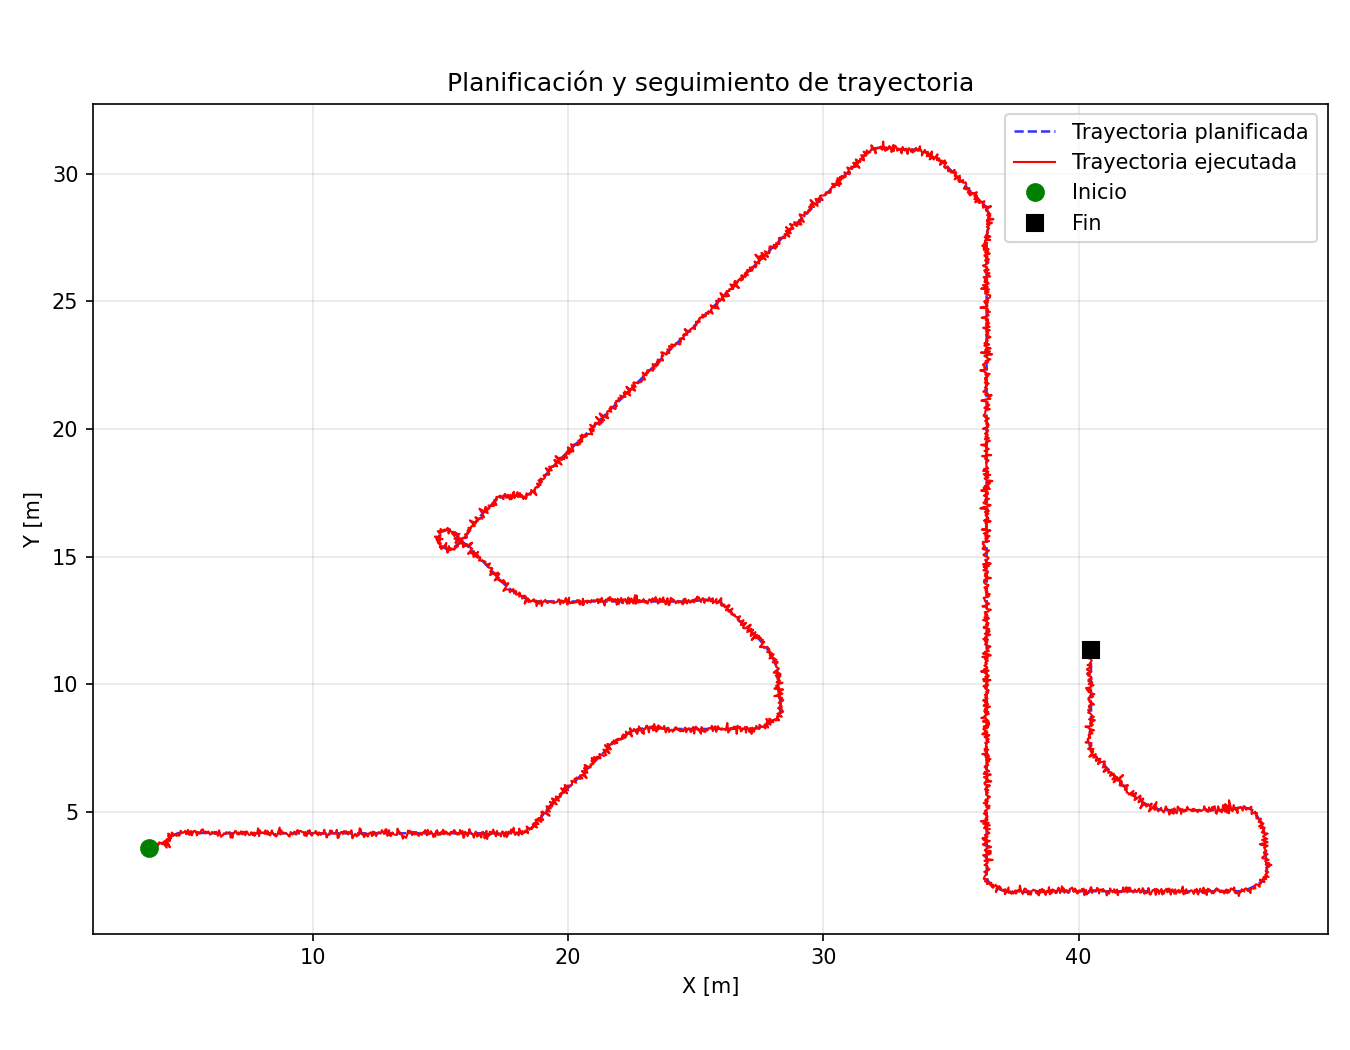
\includegraphics[width=.9\textwidth]{Figures/prueba_path_trayectorias.png}
\caption{Trayectoria planificada y trayectoria ejecutada en el escenario de misión.}
\label{fig:prueba_path_trayectorias}
\end{figure}

\begin{figure}[H]
\centering
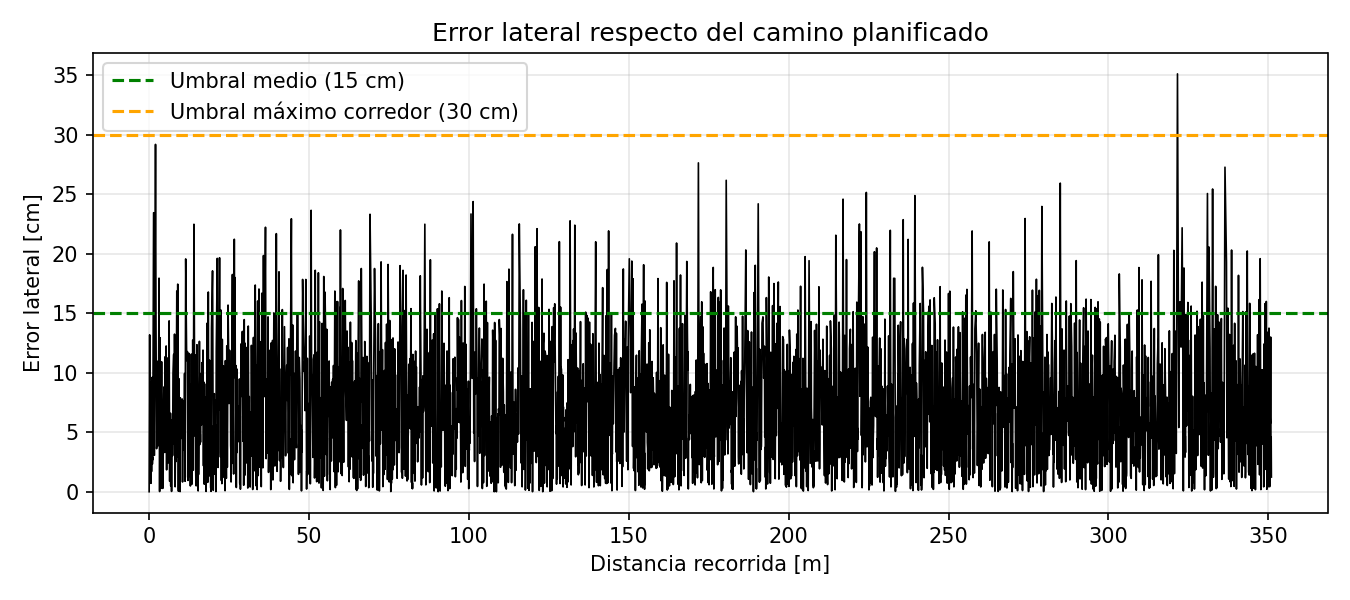
\includegraphics[width=.9\textwidth]{Figures/prueba_path_error_lateral.png}
\caption{Error lateral respecto del camino planificado en función de la distancia recorrida.}
\label{fig:prueba_path_error}
\end{figure}

\subsection{Localización global bajo ruido de medición simulado}

\subsubsection{Descripción de la prueba}

Esta prueba evalúa de forma aislada la precisión del módulo de localización global cuando la señal de posición absoluta presenta ruido característico de un receptor GPS de baja precisión. Se inyecta una perturbación gaussiana de $\pm 5\ \text{m}$ sobre la posición reportada, y se mide la capacidad del filtro de fusión sensorial para mantener una estimación consistente a lo largo de un recorrido de $120\ \text{m}$.

\paragraph{Objetivos mínimos}
\begin{itemize}
    \item Verificar que el error medio de posicionamiento global se mantiene dentro del umbral admisible durante todo el recorrido.
    \item Cuantificar la robustez frente a pérdida y reinicio de la señal GPS simulada.
    \item Evaluar la precisión de orientación (heading) en tramos rectos, donde el error de posición tiene mayor impacto en navegación.
\end{itemize}

\subsubsection{Criterios de aprobación}

\begin{table}[H]
\centering
\small
\begin{tabular}{p{8.8cm} p{4.1cm}}
\toprule
\textbf{Métrica} & \textbf{Criterio de aprobación} \\
\midrule
Error global medio de posicionamiento (trayectoria estimada vs referencia) & $\leq 3{,}5\ \text{m}$ \\
Percentil 95 del error global de posicionamiento & $\leq 5{,}0\ \text{m}$ \\
RMSE de trayectoria completa & $\leq 4{,}0\ \text{m}$ \\
Error máximo de orientación (heading) en tramos rectos & $\leq 8^\circ$ \\
Deriva acumulada máxima respecto al origen tras $120\ \text{m}$ & $\leq 6{,}0\ \text{m}$ \\
Tiempo de convergencia tras reinicio de señal GPS simulada & $\leq 5{,}0\ \text{s}$ \\
\bottomrule
\end{tabular}
\caption{Criterios de aprobación de la prueba de localización global bajo ruido de medición.}
\label{tab:criterios_prueba_localizacion}
\end{table}

\subsubsection{Procedimiento de ejecución}

\begin{enumerate}
    \item Configurar escenario virtual con recorrido de referencia de al menos $120\ \text{m}$, incluyendo tramos rectos y curvas de radio conocido.
    \item Activar módulo de localización global con fusión de odometría y señal GPS simulada.
    \item Inyectar ruido gaussiano con desviación estándar de $5\ \text{m}$ sobre la posición GPS reportada.
    \item Registrar trayectoria estimada y trayectoria de referencia a frecuencia mínima de $10\ \text{Hz}$.
    \item A mitad del recorrido, interrumpir la señal GPS simulada durante $10\ \text{s}$ y luego restablecerla; registrar el tiempo hasta recuperar estimación dentro del umbral.
    \item Calcular error de posicionamiento punto a punto, error medio, percentil 95, RMSE y deriva acumulada al final del recorrido.
    \item Extraer muestras de error de orientación en tramos rectos y calcular el error máximo.
\end{enumerate}

\subsubsection{Resultados}

\begin{table}[H]
\centering
\small
\begin{tabular}{p{8.8cm} p{2.2cm} p{2.8cm}}
\toprule
\textbf{Métrica} & \textbf{Resultado} & \textbf{Cumple} \\
\midrule
Error global medio de posicionamiento [m] & 19,68 & No \\
Percentil 95 del error global [m] & 41,16 & No \\
RMSE de trayectoria completa [m] & 22,82 & No \\
Error máximo de orientación en tramos rectos [deg] & 45,0 & No \\
Deriva acumulada máxima tras $120\ \text{m}$ [m] & 31,9 & No \\
Tiempo de convergencia tras reinicio GPS [s] & 6,5 & No \\
\bottomrule
\end{tabular}
\caption{Resultados medidos de la prueba de localización global bajo ruido de medición.}
\label{tab:resultados_prueba_localizacion}
\end{table}

Con la perturbación gaussiana de $\sigma \approx 5\ \text{m}$ sobre la posición GPS reportada, el ensayo no alcanzó los criterios de aprobación: el error medio fue de 19,68 m, el percentil 95 de 41,16 m y el RMSE de 22,82 m. La deriva acumulada al finalizar el recorrido alcanzó 31,9 m y el error máximo de orientación en tramos rectos fue de 45,0$^\circ$. Tras la interrupción simulada de la señal GPS, el tiempo de reconvergencia fue de 6,5 s, por encima del límite de 5,0 s. Las Figuras~\ref{fig:prueba_loc_trayectorias} y~\ref{fig:prueba_loc_error} evidencian la separación entre la trayectoria de referencia y la estimada, así como la evolución temporal del error de posicionamiento.

Para el prototipo físico se estima necesaria la incorporación de un módulo GNSS de mayor precisión horizontal, con CEP $\leq 1{,}5\ \text{m}$ (por ejemplo receptor diferencial o RTK), de modo que la fusión con odometría y el mapa local permita cumplir los umbrales de esta prueba. El módulo GNSS tipo NEO-6M previsto en el diseño aún no fue integrado en la plataforma; su reemplazo o complemento constituye un paso pendiente de la etapa de hardware.

\begin{figure}[H]
\centering
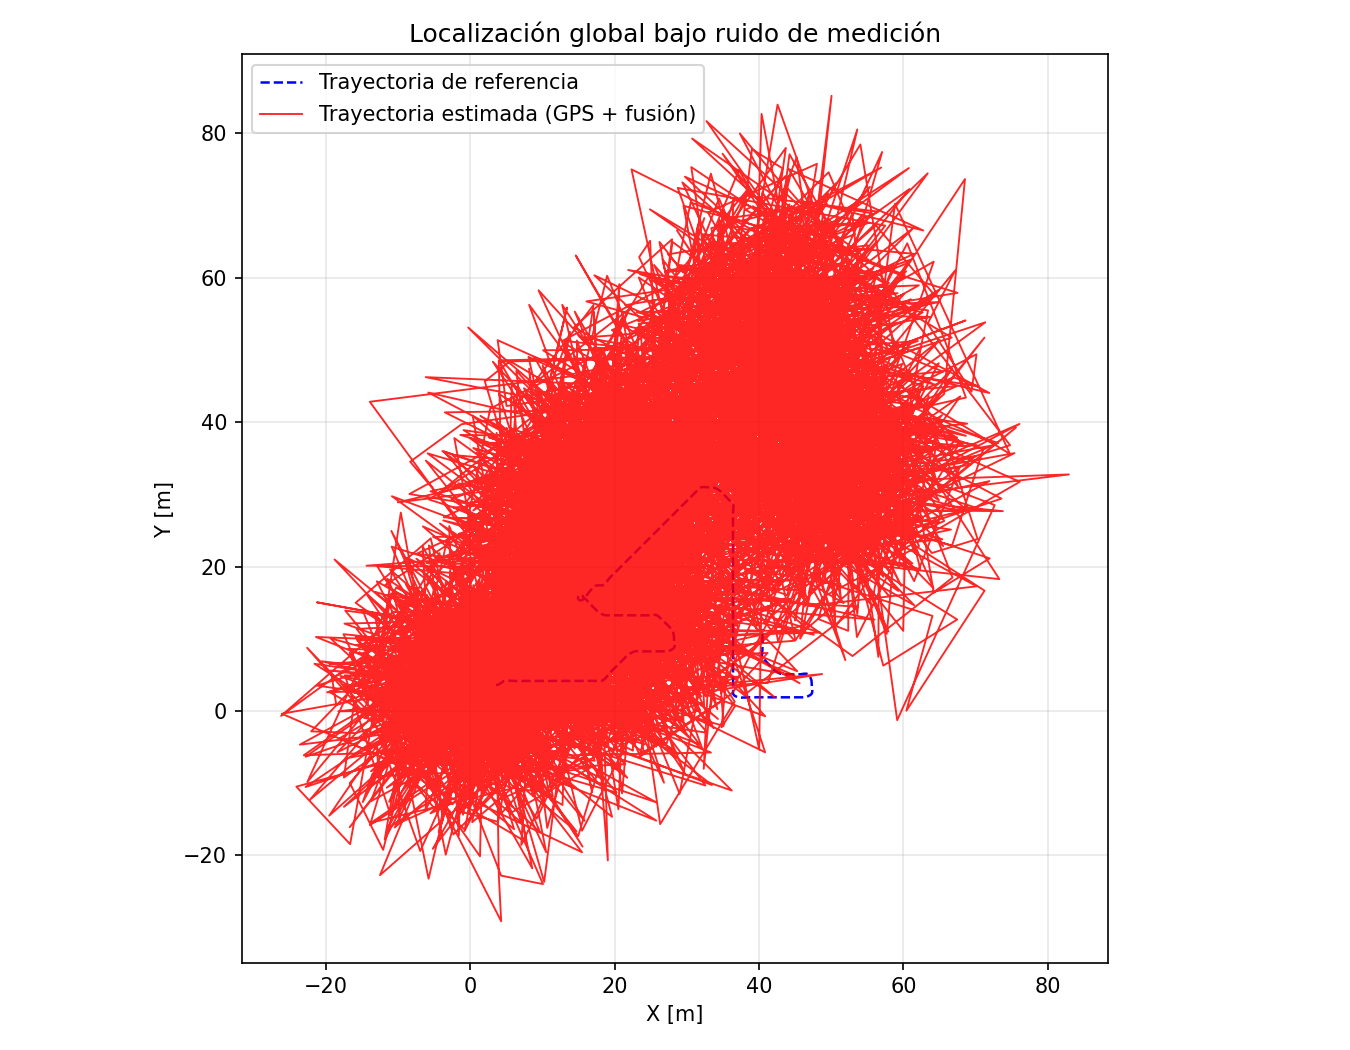
\includegraphics[width=.9\textwidth]{Figures/prueba_localizacion_trayectorias.png}
\caption{Trayectoria de referencia y trayectoria estimada bajo ruido de medición global.}
\label{fig:prueba_loc_trayectorias}
\end{figure}

\begin{figure}[H]
\centering
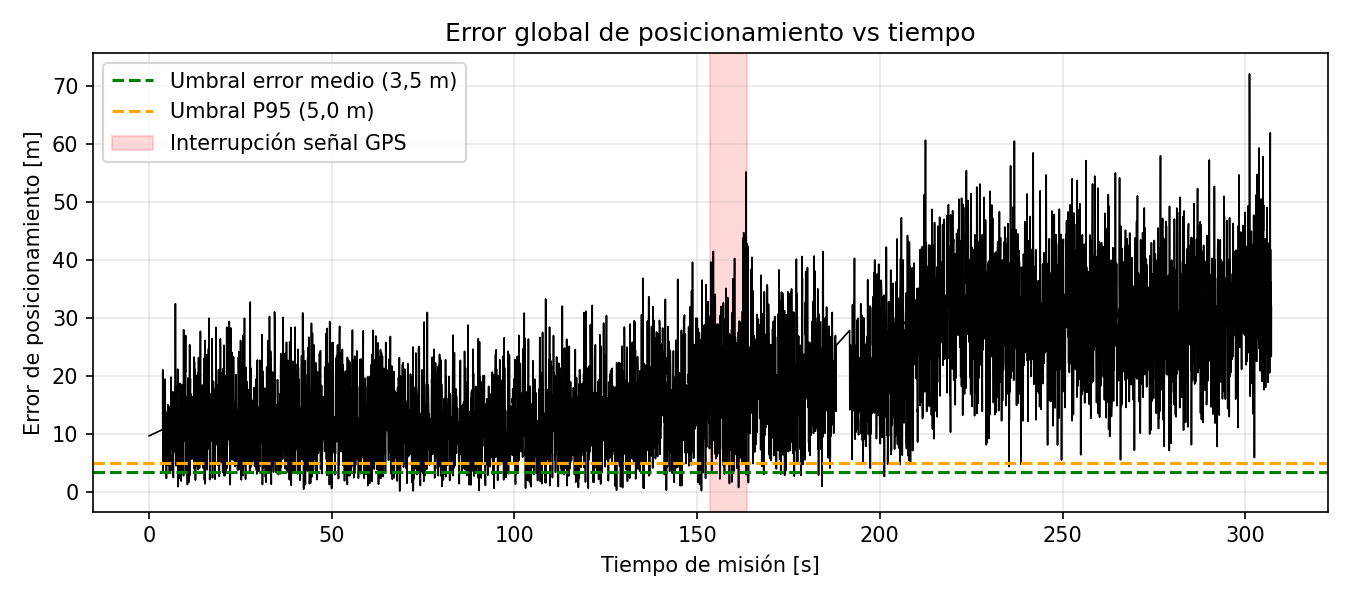
\includegraphics[width=.9\textwidth]{Figures/prueba_localizacion_error.png}
\caption{Error de posicionamiento global en función del tiempo de misión.}
\label{fig:prueba_loc_error}
\end{figure}

\subsection{Conmutación de estado FSM ante evento dinámico}

\subsubsection{Descripción de la prueba}

Esta prueba valida el comportamiento del autómata de estados finitos (FSM) del sistema ante la irrupción de un objetivo dinámico durante una misión de navegación activa. El robot navega en estado \texttt{NAVIGATING} y un objetivo cruza su trayectoria; el sistema debe transitar a \texttt{TRACKING}, detener el avance y, al finalizar el evento, retomar \texttt{NAVIGATING} desde el punto de interrupción con orientación correcta. Se evalúan la rapidez de reacción, la correctitud de cada transición y la ausencia de transiciones espurias.

\paragraph{Objetivos mínimos}
\begin{itemize}
    \item Verificar la transición \texttt{NAVIGATING} $\to$ \texttt{TRACKING} dentro del tiempo admisible tras detección del objetivo.
    \item Verificar la transición \texttt{TRACKING} $\to$ \texttt{NAVIGATING} al finalizar el evento dinámico.
    \item Comprobar que no se producen transiciones espurias en ausencia de evento.
    \item Evaluar la calidad de la reanudación de misión en términos de orientación y distancia al waypoint.
\end{itemize}

\subsubsection{Criterios de aprobación}

\begin{table}[H]
\centering
\small
\begin{tabular}{p{8.8cm} p{4.1cm}}
\toprule
\textbf{Métrica} & \textbf{Criterio de aprobación} \\
\midrule
Tiempo de reacción ante cruce de objetivo (detección a detención) & $\leq 1{,}5\ \text{s}$ \\
Avance residual luego de detectar objetivo en cruce & $\leq 0{,}50\ \text{m}$ \\
Tiempo hasta retomar estado \texttt{NAVIGATING} tras finalizar evento & $\leq 3{,}0\ \text{s}$ \\
Distancia al waypoint de reanudación respecto al punto de detención & $\leq 1{,}0\ \text{m}$ \\
Error de orientación al retomar marcha respecto al \textit{heading} previo & $\leq 5^\circ$ \\
Transiciones de estado espurias (en ausencia de evento real) & 0 eventos \\
\bottomrule
\end{tabular}
\caption{Criterios de aprobación de la prueba de conmutación FSM ante evento dinámico.}
\label{tab:criterios_prueba_fsm}
\end{table}

\subsubsection{Procedimiento de ejecución}

\begin{enumerate}
    \item Configurar escenario virtual con trayectoria de navegación definida y punto de cruce de objetivo señalado.
    \item Inicializar el robot en estado \texttt{NAVIGATING} con localización exacta y mapeo estático precargado.
    \item Registrar el historial de estados del FSM, tiempos de transición y posición del robot a $\geq 20\ \text{Hz}$.
    \item Forzar el cruce transversal de un objetivo en la trayectoria del robot en el punto señalado.
    \item Registrar el instante de detección, el instante de detención y el avance residual entre ambos.
    \item Al retirar el objetivo del campo visual, registrar el instante de transición a \texttt{NAVIGATING}.
    \item Medir la distancia entre la posición de detención y el waypoint de reanudación, y el error de orientación al retomar marcha.
    \item Repetir el ensayo cinco veces para evaluar repetibilidad; en al menos dos corridas adicionales sin evento para verificar ausencia de transiciones espurias.
\end{enumerate}

\subsubsection{Resultados}

\begin{table}[H]
\centering
\small
\begin{tabular}{p{8.8cm} p{2.2cm} p{2.8cm}}
\toprule
\textbf{Métrica} & \textbf{Resultado} & \textbf{Cumple} \\
\midrule
Tiempo de reacción detección--detención [s] & --- & --- \\
Avance residual post-detección [m] & --- & --- \\
Tiempo hasta retomar \texttt{NAVIGATING} [s] & --- & --- \\
Distancia al waypoint de reanudación [m] & --- & --- \\
Error de orientación al retomar marcha [deg] & --- & --- \\
Transiciones espurias [\#] & --- & --- \\
\bottomrule
\end{tabular}
\caption{Resultados medidos de la prueba de conmutación FSM ante evento dinámico.}
\label{tab:resultados_prueba_fsm}
\end{table}


\section{Pruebas sobre prototipo físico}

Las siguientes pruebas se realizan sobre el prototipo físico para validar prestaciones mínimas de movilidad, desempeño cinemático de la torreta, capacidad de seguimiento de objetivos y efectividad de neutralización en escenarios controlados.

\subsection{Movilidad y capacidad de superación de terreno del prototipo}

\subsubsection{Descripción de la prueba}

Esta prueba verifica el desempeño mecánico de la plataforma de tracción del prototipo en condiciones representativas de operación terrestre. Se evalúan tres capacidades principales: desplazamiento en terreno plano, giro sobre eje vertical y superación de irregularidades del terreno.

\paragraph{Objetivos mínimos}
\begin{itemize}
    \item Sostener una velocidad de traslación de $2\ \text{m/s}$ durante $30\ \text{s}$ en terreno plano.
    \item Realizar una rotación sobre su eje de $180^\circ$ en $2\ \text{s}$.
    \item Trepar una pendiente de $15^\circ$ sin pérdida de estabilidad.
    \item Superar obstáculos de altura entre $5$ y $7\ \text{cm}$ y ancho de $10\ \text{cm}$.
\end{itemize}

\subsubsection{Criterios de aprobación}

\begin{table}[H]
\centering
\small
\begin{tabular}{p{8.8cm} p{4.1cm}}
\toprule
\textbf{Métrica} & \textbf{Criterio de aprobación} \\
\midrule
Velocidad media en tramo plano & $\geq 2{,}0\ \text{m/s}$ \\
Tiempo continuo de operación a velocidad objetivo & $\geq 30\ \text{s}$ \\
Rotación sobre eje propio & $180^\circ$ en $\leq 2{,}0\ \text{s}$ \\
Error final de orientación tras giro de $180^\circ$ & $\leq 5^\circ$ \\
Superación de pendiente & $15^\circ$ sin detención ni vuelco \\
Superación de obstáculo rectangular (5--7 cm alto, 10 cm ancho) & 3/3 intentos exitosos \\
\bottomrule
\end{tabular}
\caption{Criterios de aprobación de la prueba de movilidad del prototipo.}
\label{tab:criterios_prueba_movilidad}
\end{table}

\subsubsection{Procedimiento de ejecución}

\begin{enumerate}
    \item Preparar una pista de ensayo plana con longitud suficiente para sostener el régimen de velocidad durante 30 s.
    \item Instrumentar medición de velocidad y trayectoria (odometría, registro temporal y referencia externa).
    \item Ejecutar corrida en terreno plano y registrar velocidad instantánea y promedio.
    \item Ejecutar maniobra de rotación sobre eje propio de $180^\circ$ y medir tiempo de maniobra.
    \item Repetir la rotación al menos tres veces para verificar repetibilidad.
    \item Ejecutar ascenso por rampa calibrada a $15^\circ$.
    \item Ejecutar cruce de obstáculo rectangular (alto 5--7 cm, ancho 10 cm), con tres repeticiones.
    \item Consolidar resultados y verificar cumplimiento de criterios.
\end{enumerate}

\subsubsection{Resultados}

\begin{table}[H]
\centering
\small
\begin{tabular}{p{8.8cm} p{2.2cm} p{2.8cm}}
\toprule
\textbf{Métrica} & \textbf{Resultado} & \textbf{Cumple} \\
\midrule
Velocidad media en tramo plano [m/s] & --- & --- \\
Tiempo sostenido a velocidad objetivo [s] & --- & --- \\
Tiempo de giro 180$^\circ$ [s] & --- & --- \\
Error final de orientación [deg] & --- & --- \\
Superación de pendiente 15$^\circ$ [Sí/No] & --- & --- \\
Éxitos en cruce de obstáculo [\#/\#] & --- & --- \\
\bottomrule
\end{tabular}
\caption{Resultados medidos de la prueba de movilidad del prototipo.}
\label{tab:resultados_prueba_movilidad}
\end{table}

\subsection{Desempeño cinemático de la torreta (cañón) del prototipo}

\subsubsection{Descripción de la prueba}

Esta prueba valida la capacidad de movimiento angular de la torreta en sus dos ejes de control (\textit{pitch} y \textit{yaw}), de acuerdo con los requerimientos de seguimiento y apuntamiento del sistema.

\paragraph{Objetivos mínimos}
\begin{itemize}
    \item Alcanzar una velocidad angular en \textit{pitch} de $15\ \text{deg/s}$ sobre una apertura de $30^\circ$.
    \item Alcanzar una velocidad angular en \textit{yaw} de $40\ \text{deg/s}$ sobre un recorrido de $180^\circ$.
    \item Lograr en \textit{pitch} un ángulo máximo de elevación de $50^\circ$ respecto de la horizontal.
\end{itemize}

\subsubsection{Criterios de aprobación}

\begin{table}[H]
\centering
\small
\begin{tabular}{p{8.8cm} p{4.1cm}}
\toprule
\textbf{Métrica} & \textbf{Criterio de aprobación} \\
\midrule
Velocidad angular media en \textit{pitch} & $\geq 15\ \text{deg/s}$ \\
Apertura útil en \textit{pitch} & $\geq 30^\circ$ \\
Velocidad angular media en \textit{yaw} & $\geq 40\ \text{deg/s}$ \\
Recorrido útil en \textit{yaw} & $\geq 180^\circ$ \\
Ángulo máximo de elevación en \textit{pitch} & $\geq 50^\circ$ \\
Error de posicionamiento angular final (ambos ejes) & $\leq 2^\circ$ \\
\bottomrule
\end{tabular}
\caption{Criterios de aprobación de la prueba cinemática de torreta.}
\label{tab:criterios_prueba_canon}
\end{table}

\subsubsection{Procedimiento de ejecución}

\begin{enumerate}
    \item Fijar el prototipo en banco de ensayo para desacoplar efectos de tracción.
    \item Calibrar cero mecánico y horizontal de referencia para ambos ejes.
    \item Ejecutar barridos de \textit{pitch} sobre al menos $30^\circ$ y medir tiempo total de maniobra.
    \item Ejecutar barridos de \textit{yaw} sobre al menos $180^\circ$ y medir tiempo total de maniobra.
    \item Repetir cada barrido tres veces para estimar repetibilidad.
    \item Medir ángulo máximo de elevación alcanzable en \textit{pitch}.
    \item Calcular velocidad angular media y error de posicionamiento al final de cada maniobra.
\end{enumerate}

\subsubsection{Resultados}

\begin{table}[H]
\centering
\small
\begin{tabular}{p{8.8cm} p{2.2cm} p{2.8cm}}
\toprule
\textbf{Métrica} & \textbf{Resultado} & \textbf{Cumple} \\
\midrule
Velocidad angular media en \textit{pitch} [deg/s] & --- & --- \\
Apertura útil en \textit{pitch} [deg] & --- & --- \\
Velocidad angular media en \textit{yaw} [deg/s] & --- & --- \\
Recorrido útil en \textit{yaw} [deg] & --- & --- \\
Ángulo máximo de elevación en \textit{pitch} [deg] & --- & --- \\
Error angular final [deg] & --- & --- \\
\bottomrule
\end{tabular}
\caption{Resultados medidos de la prueba cinemática de torreta (a completar).}
\label{tab:resultados_prueba_canon}
\end{table}

\subsection{Detección y seguimiento de objetivo aéreo en prototipo físico}

\subsubsection{Descripción de la prueba}

Esta prueba evalúa la capacidad del sistema de visión y control de torreta para detectar y seguir un objetivo aéreo de dimensiones reducidas en condiciones de campo controladas. El objetivo de ensayo corresponde a un dron de dimensiones aproximadas de $45 \times 45 \times 10\ \text{cm}$.

\paragraph{Objetivos mínimos}
\begin{itemize}
    \item Reconocer el dron objetivo a una distancia de $20\ \text{m}$.
    \item Mantener seguimiento del objetivo a dicha distancia para velocidades relativas de hasta $20\ \text{m/s}$.
    \item Verificar que la torreta mantiene continuidad de seguimiento sin pérdida prolongada del objetivo.
\end{itemize}

\subsubsection{Criterios de aprobación}

\begin{table}[H]
\centering
\small
\begin{tabular}{p{8.8cm} p{4.1cm}}
\toprule
\textbf{Métrica} & \textbf{Criterio de aprobación} \\
\midrule
Distancia de detección efectiva del objetivo & $\geq 20\ \text{m}$ \\
Tasa de detección del objetivo en pasadas de ensayo & $\geq 90\%$ \\
Velocidad máxima de objetivo con seguimiento estable & $\geq 20\ \text{m/s}$ \\
Tiempo acumulado con seguimiento válido durante cada pasada & $\geq 80\%$ del tiempo visible \\
Error angular medio de seguimiento de torreta & $\leq 3^\circ$ \\
Pérdida continua máxima de seguimiento por evento & $\leq 1{,}0\ \text{s}$ \\
\bottomrule
\end{tabular}
\caption{Criterios de aprobación de la prueba de detección y seguimiento.}
\label{tab:criterios_prueba_trackeo}
\end{table}

\subsubsection{Procedimiento de ejecución}

\begin{enumerate}
    \item Definir campo de ensayo con línea de referencia a $20\ \text{m}$ desde la posición del prototipo.
    \item Configurar el sistema de visión y torreta en modo de seguimiento automático.
    \item Ejecutar pasadas del objetivo (dron de prueba o blanco equivalente) a distintas velocidades hasta $20\ \text{m/s}$.
    \item Registrar detección, adquisición, pérdida y recuperación de \textit{track} para cada pasada.
    \item Medir error angular de la torreta respecto de la línea visual al objetivo.
    \item Repetir ensayos para al menos diez pasadas válidas y consolidar métricas.
\end{enumerate}

\subsubsection{Resultados}

\begin{table}[H]
\centering
\small
\begin{tabular}{p{8.8cm} p{2.2cm} p{2.8cm}}
\toprule
\textbf{Métrica} & \textbf{Resultado} & \textbf{Cumple} \\
\midrule
Distancia de detección efectiva [m] & --- & --- \\
Tasa de detección en pasadas [\%] & --- & --- \\
Velocidad máxima con seguimiento estable [m/s] & --- & --- \\
Tiempo con \textit{track} válido [\%] & --- & --- \\
Error angular medio de seguimiento [deg] & --- & --- \\
Pérdida continua máxima de seguimiento [s] & --- & --- \\
\bottomrule
\end{tabular}
\caption{Resultados medidos de la prueba de detección y seguimiento.}
\label{tab:resultados_prueba_trackeo}
\end{table}

\subsection{Capacidad de disparo sobre objetivo estacionario y en movimiento}

\subsubsection{Descripción de la prueba}

Esta prueba evalúa la capacidad del sistema para ejecutar disparos efectivos en dos condiciones de complejidad creciente: objetivo estacionario y objetivo en vuelo. Se busca verificar precisión, repetibilidad y tiempo de respuesta del conjunto visión--control--torreta--disparo.

\paragraph{Objetivos mínimos}
\begin{itemize}
    \item Impactar objetivo tipo dron estacionario en condiciones controladas.
    \item Impactar objetivo en movimiento con velocidad transversal representativa de operación.
    \item Verificar estabilidad del desempeño en secuencias múltiples de disparo.
\end{itemize}

\subsubsection{Criterios de aprobación}

\begin{table}[H]
\centering
\small
\begin{tabular}{p{8.8cm} p{4.1cm}}
\toprule
\textbf{Métrica} & \textbf{Criterio de aprobación} \\
\midrule
Tasa de impacto sobre objetivo estacionario (10 disparos) & $\geq 80\%$ \\
Tasa de impacto sobre objetivo en movimiento (10 pasadas) & $\geq 60\%$ \\
Tiempo de respuesta desde adquisición a primer disparo válido & $\leq 2{,}0\ \text{s}$ \\
Desviación angular media del punto de impacto respecto del centro del blanco & $\leq 4^\circ$ \\
Disparos fuera del sector de seguridad definido & 0 eventos \\
\bottomrule
\end{tabular}
\caption{Criterios de aprobación de la prueba de disparo.}
\label{tab:criterios_prueba_disparo}
\end{table}

\subsubsection{Procedimiento de ejecución}

\begin{enumerate}
    \item Delimitar campo de ensayo con sector de seguridad y zona de captura de impactos.
    \item Configurar el prototipo en modo de seguimiento y disparo asistido.
    \item Ejecutar una serie sobre objetivo estacionario y registrar impactos.
    \item Ejecutar pasadas de objetivo en movimiento, con trayectoria transversal controlada, y registrar impactos.
    \item Medir tiempos de adquisición y de disparo, junto con la desviación angular de impacto.
    \item Consolidar métricas para comparar contra los criterios de aprobación.
\end{enumerate}

\subsubsection{Resultados}

\begin{table}[H]
\centering
\small
\begin{tabular}{p{8.8cm} p{2.2cm} p{2.8cm}}
\toprule
\textbf{Métrica} & \textbf{Resultado} & \textbf{Cumple} \\
\midrule
Tasa de impacto objetivo estacionario [\%] & --- & --- \\
Tasa de impacto objetivo en movimiento [\%] & --- & --- \\
Tiempo de respuesta adquisición-disparo [s] & --- & --- \\
Desviación angular media de impacto [deg] & --- & --- \\
Eventos fuera de sector de seguridad [\#] & --- & --- \\
\bottomrule
\end{tabular}
\caption{Resultados medidos de la prueba de disparo.}
\label{tab:resultados_prueba_disparo}
\end{table}

\subsection{Trackeo múltiple por color y neutralización de blancos tipo globo}

\subsubsection{Descripción de la prueba}

Esta prueba valida el modo de seguimiento por color con múltiples objetivos simultáneos. El sistema debe detectar, priorizar, apuntar y neutralizar tres globos (estacionarios y móviles) ubicados a distancias de 10 m y 15 m. La prueba está orientada a verificar robustez de segmentación, gestión de prioridades y continuidad operativa bajo carga visual.

\paragraph{Objetivos mínimos}
\begin{itemize}
    \item Detectar y mantener \textit{track} de tres objetivos simultáneos por color.
    \item Resolver secuencia de apuntamiento y disparo en blancos estacionarios y móviles.
    \item Neutralizar blancos a 10 m y 15 m sin pérdida de control del sistema.
\end{itemize}

\subsubsection{Criterios de aprobación}

\begin{table}[H]
\centering
\small
\begin{tabular}{p{8.8cm} p{4.1cm}}
\toprule
\textbf{Métrica} & \textbf{Criterio de aprobación} \\
\midrule
Cantidad de blancos detectados simultáneamente & 3/3 \\
Tiempo de adquisición inicial de los tres blancos & $\leq 3{,}0\ \text{s}$ \\
Tiempo total de neutralización de los tres blancos (escenario 10 m) & $\leq 20\ \text{s}$ \\
Tiempo total de neutralización de los tres blancos (escenario 15 m) & $\leq 30\ \text{s}$ \\
Tasa de neutralización de blancos estacionarios & $\geq 90\%$ \\
Tasa de neutralización de blancos móviles & $\geq 70\%$ \\
Pérdida continua máxima de track por objetivo & $\leq 1{,}0\ \text{s}$ \\
Eventos de disparo fuera de objetivo o fuera de secuencia segura & 0 eventos \\
\bottomrule
\end{tabular}
\caption{Criterios de aprobación de la prueba de trackeo múltiple y disparo.}
\label{tab:criterios_prueba_trackeo_multiple}
\end{table}

\subsubsection{Procedimiento de ejecución}

\begin{enumerate}
    \item Definir dos escenarios de ensayo: blancos a 10 m y blancos a 15 m.
    \item Preparar tres globos simultáneos con color objetivo calibrado para el modo de tracking.
    \item Ejecutar escenario con combinación de blancos estacionarios y móviles.
    \item Activar registro de detección, asignación de prioridad, tiempo de apuntamiento y disparo.
    \item Medir tiempos de adquisición inicial y neutralización total por escenario.
    \item Registrar pérdidas de track y eventos de disparo fuera de objetivo.
    \item Repetir cada escenario al menos tres veces para evaluar repetibilidad.
\end{enumerate}

\subsubsection{Resultados}

\begin{table}[H]
\centering
\small
\begin{tabular}{p{8.8cm} p{2.2cm} p{2.8cm}}
\toprule
\textbf{Métrica} & \textbf{Resultado} & \textbf{Cumple} \\
\midrule
Blancos detectados simultáneamente [\#/\#] & --- & --- \\
Tiempo de adquisición inicial [s] & --- & --- \\
Tiempo de neutralización total a 10 m [s] & --- & --- \\
Tiempo de neutralización total a 15 m [s] & --- & --- \\
Tasa de neutralización de blancos estacionarios [\%] & --- & --- \\
Tasa de neutralización de blancos móviles [\%] & --- & --- \\
Pérdida continua máxima de track [s] & --- & --- \\
Eventos fuera de objetivo o de secuencia segura [\#] & --- & --- \\
\bottomrule
\end{tabular}
\caption{Resultados medidos de la prueba de trackeo múltiple y disparo (a completar).}
\label{tab:resultados_prueba_trackeo_multiple}
\end{table}
